\documentclass[]{article}
\newcommand{\FileDepth}{../../..}
\usepackage[letterpaper, landscape, margin=0.5cm]{geometry}
\usepackage[T1]{fontenc}
\usepackage{textcomp}%Not strictly necessary, but gives \textmu command for "micro."
\usepackage{fancyhdr}
\usepackage{amsmath}
\usepackage{amssymb}
\usepackage{graphicx}
\usepackage{xcolor}
\usepackage{tikz}
\usetikzlibrary{calc}
\usepackage[shortlabels]{enumitem}
\usepackage{multicol}
\usepackage{vwcol}
\usepackage{hyperref}
\usepackage{wrapfig}
%opening
\newcommand{\SecType}{L}
\newcommand{\Week}{13}
\title{PH 211 Lecture \Week}
\author{Benjamin Bauml}
\date{Summer 2024}

\newcommand{\Purpose}{4}
\newcommand{\DefOnly}{0}

% Version 2024-06-14
% Changes
% 2024-02-21 Added xstring package to enable smooth implementation of new \ModePage command.
% 2024-04-27 Set up to split activities and formatting aspects into separate files. Removed dependence on xcomment. Added an automatic counter to number the activities in a problem set.
% 2024-05-19 Revised old format for \TeachingTips command, which did not support \DefOnly.
% 2024-06-14 Added Repurpose environment to allow mixing of different purpose levels in the same document.
\usepackage{tcolorbox}
\usepackage{xstring}
% You will want the following four lines in your document (the last two uncommented):
% For Assignment, leave Purpose as 1. For Worksheet, set to 2. For Student Solution, set to 3. For Teacher Solution, set to 4.
% If you want keep the pieces from being called manually, set DefOnly to 0.
%\newcommand{\Purpose}{4}
%\newcommand{\DefOnly}{1}
\newcommand{\Exclusion}{0}
\newcommand{\PageTurn}{0}
\newcommand{\GrayProb}{0}
\newcommand{\Tipsy}{0}

% Assignment
\if\Purpose1
\renewcommand{\Exclusion}{1}
\fi
% Worksheet
\if\Purpose2
\renewcommand{\Exclusion}{1}
\renewcommand{\PageTurn}{1}
\fi
% Student Solution
\if\Purpose3
\renewcommand{\PageTurn}{1}
\renewcommand{\GrayProb}{1}
\fi
% Teaching Copy
\if\Purpose4
\renewcommand{\PageTurn}{1}
\renewcommand{\GrayProb}{1}
\renewcommand{\Tipsy}{1}
\fi

\newenvironment{Repurpose}[1]{
\renewcommand{\Purpose}{#1}
\renewcommand{\Exclusion}{0}
\renewcommand{\PageTurn}{0}
\renewcommand{\GrayProb}{0}
\renewcommand{\Tipsy}{0}
% Assignment
\if\Purpose1
\renewcommand{\Exclusion}{1}
\fi
% Worksheet
\if\Purpose2
\renewcommand{\Exclusion}{1}
\renewcommand{\PageTurn}{1}
\fi
% Student Solution
\if\Purpose3
\renewcommand{\PageTurn}{1}
\renewcommand{\GrayProb}{1}
\fi
% Teaching Copy
\if\Purpose4
\renewcommand{\PageTurn}{1}
\renewcommand{\GrayProb}{1}
\renewcommand{\Tipsy}{1}
\fi
}{}

\def \NewQ {0}
\def \PForce {0}
\newcommand{\MaybePage}[1]{
	\def \PForce {#1}
	\if\PForce1
	\newpage
	\else
	\if\NewQ0
	\gdef \NewQ {\PageTurn}
	\else
	\newpage
	\fi
	\fi
}

\newcommand{\ModePage}[1]{
	\IfSubStr{#1}{\Purpose}{\newpage}{}
}

\newcounter{ActNumber}
\setcounter{ActNumber}{0}

\newcommand{\Problem}[4][0]{%The first argument is optional, and if it is set to 1, the \newpage will be forced. The second argument is the name of the activity, the third is the command the activity is stored as, and the fourth is the actual problem statement.
\newcommand{#3}{
\MaybePage{#1}
\addtocounter{ActNumber}{1}
\section*{\SecType\Week-\theActNumber: #2}
\if\GrayProb1
\begin{tcolorbox}[colback=lightgray,colframe=lightgray,sharp corners,boxsep=1pt,left=0pt,right=0pt,top=0pt,bottom=0pt,after skip=2pt]
\else
\begin{tcolorbox}[colback=white,colframe=white,sharp corners,boxsep=1pt,left=0pt,right=0pt,top=0pt,bottom=0pt,after skip=2pt]
\fi
#4
\end{tcolorbox}\noindent
}
\if\DefOnly0
\else
#3
\fi
}
	
\newcommand{\ProblemSub}[3][0]{%The first argument is optional, and if a string of numbers is entered into it, it will force a \newpage in any \Purpose that shows up in the string. For example, "13" would lead to the newpage being forced in modes 1 and 3. The second is the command the activity is stored as, and the third is the actual problem statement.
\newcommand{#2}{
\ModePage{#1}
\if\GrayProb1
\begin{tcolorbox}[colback=lightgray,colframe=lightgray,sharp corners,boxsep=1pt,left=0pt,right=0pt,top=0pt,bottom=0pt,after skip=2pt]
\else
\begin{tcolorbox}[colback=white,colframe=white,sharp corners,boxsep=1pt,left=0pt,right=0pt,top=0pt,bottom=0pt,after skip=2pt]
\fi
#3
\end{tcolorbox}\noindent
}
\if\DefOnly0
\else
#2
\fi
}
		
\newcommand{\Solution}[2]{%The first argument is the command the solution is stored as, and the second is the actual solution.
\newcommand{#1}{
\if\Exclusion0
#2
\fi
}
\if\DefOnly0
\else
#1
\fi
}
		
\newcommand{\ProblemFig}[2]{%The first argument is the command the figure is stored as, and the second is the actual figure.
\newcommand{#1}{
\begin{figure}[h]
#2
\end{figure}
}
\if\DefOnly0
\else
#1
\fi
}

\newcommand{\TeachingTips}[2]{%The first argument is the command the tip is stored as, and the second is the actual tip.
\newcommand{#1}{
\if\Tipsy1
\begin{tcolorbox}[colback=lightgray,colframe=black]
#2
\end{tcolorbox}
\fi
}
\if\DefOnly0
\else
#1
\fi
}
\usepackage[absolute]{textpos}
% This package relies on Assignment Format 2024-06-14 or later to work. It is recommended that the Purpose and DefOnly commands be given as such:
%\newcommand{\Purpose}{4}
%\newcommand{\DefOnly}{0}
% Activities need to be entered outside of the TeacherMargin and PresentSpace environments, otherwise they will be defined only locally. They can even go in the preamble.
\newenvironment{TeacherMargin}{\begin{textblock*}{10.8cm}(0.5cm,0.5cm)
\small}{\end{textblock*}
\hspace{0.1cm}}
\newenvironment{PresentSpace}{\begin{textblock*}{0.3cm}(26.85cm,9.35cm)
--
\end{textblock*}
\begin{textblock*}{0.3cm}(26.85cm,18.7cm)
--
\end{textblock*}
\begin{textblock*}{0.3cm}(26.85cm,12.24cm)
	--
\end{textblock*}
\begin{textblock*}{15.6cm}(11.8cm,0.5cm)
\begin{Repurpose}{1}
\Large}{\end{Repurpose}
\end{textblock*}
\hspace{0.1cm}}

\newcommand{\FBDaxes}[3]{
	\begin{scope}[shift={(#1)},rotate=#2]
		% x-axis
		\draw[thick,->] (-2,0) -- (2,0);
		\node[anchor=west] at (2,0) {$x$};
		% y-axis
		\draw[thick,->] (0,-2) -- (0,2);
		\node[anchor=west] at (0,2) {$y$};
		\coordinate (#3) at (0,0);
	\end{scope}
}
\newcommand{\FBDvectorMA}[4]{
	\begin{scope}[shift={(#1)}]
		\coordinate (#4tip) at ({#2*cos(#3)},{#2*sin(#3)});
		\draw[ultra thick,blue,->] (#1) -- (#4tip);
	\end{scope}
}
\newcommand{\FBDvectorXY}[3]{
	\begin{scope}[shift={(#1)}]
		\coordinate (#3tip) at (#2);
		\draw[ultra thick,blue,->] (0,0) -- (#3tip);
	\end{scope}
}
\newcommand{\FBDdot}[1]{
	\filldraw[black] (#1) circle (3pt);
}
%\newcommand{\MVec}[3][0]{%Creates a momentum vector of length #3 centered at #2 and rotated #1 degrees counterclockwise.
	\begin{scope}[rotate=#1,shift={(#2)}]
		\draw[->,thick] ({-#3/2},0) -- ({#3/2},0);
	\end{scope}
}
\newcommand{\MDot}[1]{%Creates a dot at #1 to represent a zero vector.
	\filldraw (#1) circle (1pt);
}
\newcommand{\MVDRows}[2][4.5]{%Creates the rows (initial, delta, final) of a momentum vector diagram. The optional argument determines the width of the table, and defaults to a good length for three columns (two objects and the total system). The non-optional argument gives a coordinate name (not displayed) to the diagram.
	\begin{scope}
		%\draw[thick] (0,5.5) -- (0,0);
		\draw[thick] (-1,4.5) -- (#1,4.5);
		\node at (-0.5,3.75) {$\vec{p}_{i}$};
		\draw[thick] (-1,3) -- (#1,3);
		\node at (-0.5,2.25) {$\Delta\vec{p}$};
		\draw[thick] (-1,1.5) -- (#1,1.5);
		\node at (-0.5,0.75) {$\vec{p}_{f}$};
		\coordinate (#2) at (0,5);
	\end{scope}
}
\newcommand{\MVDCol}[4][0.75]{%Creates a column for an object in a momentum vector diagram. The first (non-optional) argument is the coordinate name (not displayed) of the column, while the second is the displayed column header. The first argument also names the three entries down the column. The third argument anchors the column, so it should either be the coordinate name of the MVD (for the first column) or the coordinate name of the previous column. The optional argument indicates how far the center of the column should be from the previous column's edge, and defaults to 0.75
	\begin{scope}[shift={(#4)}]
		\node at (#1,0) {#3};
		%\draw[thick] ({#1*2},0.5) -- ({#1*2},-5);
		\draw[thick] (0,0.5) -- (0,-5);
		\coordinate (#2init) at (#1,-1.25);
		\coordinate (#2delt) at (#1,-2.75);
		\coordinate (#2fin) at (#1,-4.25);
		\coordinate (#2) at ({#1*2},0);
	\end{scope}
}

%\input{\FileDepth/Activities/Activity_One/Activity_One.tex}
%\input{\FileDepth/Activities/Activity_Two/Activity_Two.tex}

\begin{document}
\begin{TeacherMargin}

\end{TeacherMargin}
\begin{PresentSpace}
\begin{center}
	\huge Lecture \Week: Newton' 3rd Law of Motion \\
	\small (and a Bit of Springs)
\end{center}
\vspace{0.5cm}
\underline{Warm-Up Activity} \\
Which of the following statements, if any, are true about Newton's 3rd law pairs?
\begin{enumerate}[(A)]
	\item They appear on different free-body diagrams.
	\item They are the same type of force.
	\item They appear on the same free-body diagram.
	\item $\vec{F}^{t}_{AB} = -\vec{F}^{t}_{AB}$
\end{enumerate}
\vspace{1cm}
\underline{Feedback Question} \\
Do you prefer feedback through documents uploaded to Canvas, or through Gradescope (as was done on the quizzes)?
%\begin{multicols}{2}
\begin{enumerate}[(A)]
	\item PDFs on Canvas
	\item Comments in Gradescope
\end{enumerate}
%\end{multicols}
\end{PresentSpace}
\newpage
\begin{TeacherMargin}

\end{TeacherMargin}
\begin{PresentSpace}
\vspace{-10pt}
\section*{Newton's 3rd Law of Motion}
\vspace{-10pt}
\begin{itemize}
	\item If A exerts a force on B, then B exerts a force of the same magnitude on A in the opposite direction:
	\[
	\vec{F}^{t}_{AB} = -\vec{F}^{t}_{BA}
	\]
	\item These two forces make a \textit{Newton's 3rd law pair}, or an \textit{action-reaction pair}.
	\item 3rd law pair forces\dots
	\begin{itemize}
		\item are the same type of force;
		\item appear on different free body diagrams.
	\end{itemize}
\end{itemize}
\end{PresentSpace}
\newpage
\begin{TeacherMargin}
\noindent\textbf{The Negative Sign} \\
The negative sign tells us that the force of the spring points opposite the displacement from equilibrium. The spring wants to return to its \\
unstretched/uncompressed length. Forces that try to return a system to equilibrium are called \textit{restoring forces}.
\end{TeacherMargin}
\begin{PresentSpace}
\vspace{-10pt}
\section*{Spring Forces}
\vspace{-10pt}
\begin{itemize}
	\item Many objects resist changes in physical configuration (\textit{i.e.} deformations).
	\item For small deformations, we can model the object as a spring.
	\item The forces caused by springs obey Hooke's law: $\vec{F}^{S} = -k(\vec{x}-\vec{x}_{eq})$.
	\begin{itemize}
		\item $\Delta\vec{x} = (\vec{x}-\vec{x}_{eq})$ is displacement from equilibrium.
		\item $k$ is the spring constant.
		\item What does the negative sign mean?
	\end{itemize}
\end{itemize}
\end{PresentSpace}
\newpage
\begin{TeacherMargin}

\end{TeacherMargin}
\begin{PresentSpace}
\vspace{-10pt}
\section*{Types of Forces}
\vspace{-10pt}
\begin{itemize}
	\item Gravity \qquad \qquad \qquad \qquad $\vec{F}^{g}_{AB} = m_{A}\vec{g}_{B}$
	\begin{itemize}
		\item Newtonian \qquad\ $\vec{g}_{B} = G\frac{M_{B}}{r^{2}}(-\hat{r})$, $G = 6.67408\times10^{-11}\text{ N}\cdot\text{m}^{2}/\text{kg}^{2}$
		\item Near-Earth \qquad $\vec{g}_{E} = g(-\hat{y}),\ g=9.81\frac{\text{m}}{\text{s}^{2}} \approx 10\frac{\text{m}}{\text{s}^{2}}$
	\end{itemize}
	\item Normal \qquad $\vec{F}^{N}$ always $\bot$; varies in magnitude
	\item Tension \qquad $\vec{F}^{T}$ uniform (massless, inextensible rope)
	\item Spring \qquad $\vec{F}^{S}=-k(\vec{x}-\vec{x}_{eq})$
	\item Friction
	\begin{itemize}
		\item Static Friction \qquad $F^{sf}\leq\mu_{s}|\vec{F}^{N}|$
		\item Kinetic Friction \qquad $F^{kf}=\mu_{k}|\vec{F}^{N}|$
	\end{itemize}
\end{itemize}
\end{PresentSpace}
\begin{textblock*}{5cm}(22cm,6cm)
	\Large
	\noindent\textbf{Not Forces}
	\begin{itemize}
		\normalsize
		\item Momentum
		\item Inertia
		\item Velocity
		\item Acceleration
	\end{itemize}
\end{textblock*}
\newpage
\begin{TeacherMargin}

\end{TeacherMargin}
\begin{PresentSpace}
\vspace{-10pt}
\section*{A*R*C*S: Uh-Oh Dr. Paws}
%\vspace{-10pt}
In the video in Section 3.16 of our textbook, Paul \\
pushes a footstool (mass $m_{1}$) across the floor with \\
a constant force so that the footstool speeds up. \\
Dr. Paws (a dog with mass $m_{2}$) is sitting on the \\
footstool. The coefficient of static friction between \\
the dog and the footstool is $\mu$ (assume no friction \\
between the footstool and the ground). How much \\
force can Paul exert on the footstool before the dog \\
begins sliding?
\end{PresentSpace}
\begin{textblock*}{4cm}(23cm,2cm)
	\Large
	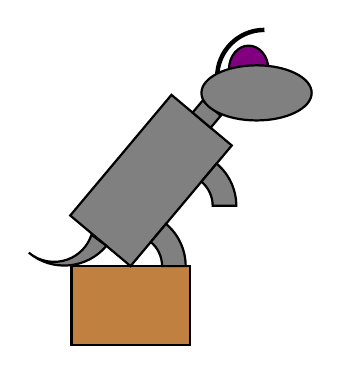
\begin{tikzpicture}
		\draw[thick,color=black,fill=brown] (-0.75,0) rectangle (0.75,1);
		\begin{scope}[shift={(0,1)}]
			\draw[thick,color=black,fill=gray,rotate=50] (0,0) rectangle (2,1);
			\draw[thick,color=black,fill=gray,rotate=50] (0,0.4) arc (270:180:0.7) arc (180:292:0.5) -- cycle;
			\draw[thick,color=black,fill=gray,rotate=50] (0.4,0) arc (0:-50:0.4) -- ({0.7*cos(50)},{-0.7*sin(50)}) arc (310:360:0.7) -- cycle;
			\draw[thick,color=black,fill=gray,rotate=50,shift={(1,0)}] (0.4,0) arc (0:-50:0.4) -- ({0.7*cos(50)},{-0.7*sin(50)}) arc (310:360:0.7) -- cycle;
			\draw[thick,color=black,fill=gray,rotate=50] (2,0.65) -- (2.2,0.65) -- (2.2,0.35) -- (2,0.35) -- cycle;
			\draw[ultra thick,black] (1.1,2.4) arc (180:90:0.6);
			\draw[thick,color=black,fill=violet] (1.5,2.5) circle (0.25 and 0.3);
			\draw[thick,color=black,fill=gray] (1.6,2.2) ellipse (0.7 and 0.35);
		\end{scope}
	\end{tikzpicture}
\end{textblock*}
\newpage
\begin{TeacherMargin}
\noindent\textbf{(1a) Understand the Problem}
\begin{itemize}
	\item Mass of the dog: $m_{2}=30\text{ kg}$
	\begin{itemize}
		\item A typical golden retriever is 25-34 kg, so a nice round 30 kg is reasonable and helpful to us.
	\end{itemize}
	\item Mass of the footstool: $m_{1}=10\text{ kg}$
	\begin{itemize}
		\item A footstool can reasonably have less mass than a sizable dog.
	\end{itemize}
	\item Gravity: $g=10\text{ m/s}^{2}$
	\begin{itemize}
		\item This comes from our near-Earth approximation.
	\end{itemize}
	\item Coefficient of static friction: $\mu=0.4$
	\begin{itemize}
		\item This is a reasonable coefficient of static friction in general (wood-on-wood can range from 0.25-0.5, by some sources), and I don't have a better guess for the specific situation of dog-on-footstool.
	\end{itemize}
\end{itemize}
\textbf{(1b) Identify Assumptions}
%\begin{multicols}{2}
\begin{itemize}
	\item Near-Earth
	\begin{itemize}
		\item This can reasonably be expected to occur in a home on Earth's surface, where elevation does not appreciably affect gravitational acceleration.
	\end{itemize}
	\item Neglect air-resistance
	\begin{itemize}
		\item Air resistance is a much weaker effect at low speeds, and we probably are not going to get the dog truly racing in our living room.
	\end{itemize}
	\item Dr. Paws doesn't move.
	\begin{itemize}
		\item This is probably the weakest assumption (we saw what Dr. Paws did in the video), but it is necessary, as the problem becomes far more difficult if the dog and the stool do not move perfectly together. With this, we can say that $\vec{a}_{D} = \vec{a}_{S} = a\hat{x}$.
	\end{itemize}
	\item Particle model
	\begin{itemize}
		\item If the dog doesn't move, then its shape doesn't change, and it doesn't rotate, so we can ignore those complicated aspects of motion and just concentrate on the motion of the dog's center of mass.
	\end{itemize}
\end{itemize}
%\end{multicols}
\textbf{(1c) Represent Physically}
%\begin{multicols}{2}
\begin{center}
	\begin{tikzpicture}
		\FBDaxes{0,0}{0}{dogaxes}
		\FBDbox[0.6]{dogaxes}{0}{dogbox}{$D$}
		\FBDvectorXY{dogboxtcent}{0,1}{FNDS}
		\node[anchor=east] at (FNDStip) {$\vec{F}^{N}_{DS}$};
		\FBDvectorXY{dogboxbcent}{0,-1}{FGDE}
		\node[anchor=east] at (FGDEtip) {$\vec{F}^{g}_{DE}$};
		\FBDvectorXY{dogboxrcent}{1,0}{FSFDS}
		\node[anchor=south] at (FSFDStip) {$\vec{F}^{sf}_{DS}$};
		\FBDaxes{5,0}{0}{stoolaxes}
		\FBDbox[0.6]{stoolaxes}{0}{stoolbox}{$S$}
		\FBDvectorXY{stoolboxtcent}{0,1.33}{FNSG}
		\node[anchor=west] at (FNSGtip) {$\vec{F}^{N}_{SG}$};
		\FBDvectorXY{stoolboxblq}{0,-1}{FNSD}
		\node[anchor=east] at (FNSDtip) {$\vec{F}^{N}_{SD}$};
		\FBDvectorXY{stoolboxbrq}{0,-0.33}{FGSE}
		\node[anchor=west] at (FGSEtip) {$\vec{F}^{g}_{SE}$};
		\FBDvectorXY{stoolboxlcent}{-1,0}{FSFTSD}
		\node[anchor=south] at (FSFTSDtip) {$\vec{F}^{sf}_{SD}$};
		\FBDvectorXY{stoolboxrcent}{1.33,0}{FNSP}
		\node[anchor=south] at (FNSPtip) {$\vec{F}^{N}_{SP}$};
		\node[anchor=north west] at (0.75,2.25) {\parbox{4cm}{Our 3rd law pairs are
				\begin{itemize}
					\item $\vec{F}^{N}_{DS}$ and $\vec{F}^{N}_{SD}$;
					\item $\vec{F}^{sf}_{DS}$ and $\vec{F}^{sf}_{SD}$.
		\end{itemize}}};
		\node[anchor=north west] at (0.75,-0.25) {\parbox{3cm}{(The vectors in each of these pairs were not equal in magnitude in the diagrams on the right.)}};
	\end{tikzpicture}
\end{center}
%\end{multicols}
\end{TeacherMargin}
\begin{PresentSpace}
\vspace{-10pt}
\section*{L\Week-1: Uh-Oh Dr. Paws -- Analyze and Represent}
\vspace{-20pt}
\begin{multicols}{2}
	\textbf{(1a) Understand the Problem}
	\begin{itemize}
		\large
		\item Mass of the footstool: $m_{1}=10\text{ kg}$
		\item Mass of the dog: $m_{2}=30\text{ kg}$
		\item Gravity: $g=10\text{ m/s}^{2}$
		\item Coefficient of static friction: $\mu=0.4$
	\end{itemize}
	\textbf{(1b) Identify Assumptions}
	\begin{itemize}
		\large
		\item Near-Earth
		\item Particle model
		\item Neglect air-resistance
		\item Dr. Paws doesn't move.
	\end{itemize}
	\textbf{(1c) Represent Physically}
	\begin{center}
		\begin{tikzpicture}
			\FBDaxes{0,0}{0}{dogaxes}
			\FBDbox[0.6]{dogaxes}{0}{dogbox}{$D$}
			\FBDvectorXY{dogboxtcent}{0,1}{FNDS}
			\node[anchor=east] at (FNDStip) {$\vec{F}^{N}_{DS}$};
			\FBDvectorXY{dogboxbcent}{0,-1}{FGDE}
			\node[anchor=east] at (FGDEtip) {$\vec{F}^{g}_{DE}$};
			\FBDvectorXY{dogboxrcent}{1.5,0}{FSFDS}
			\node[anchor=south] at (FSFDStip) {$\vec{F}^{sf}_{DS}$};
			\FBDaxes{3,-2}{0}{stoolaxes}
			\FBDbox[0.6]{stoolaxes}{0}{stoolbox}{$S$}
			\FBDvectorXY{stoolboxtcent}{0,1.33}{FNSG}
			\node[anchor=west] at (FNSGtip) {$\vec{F}^{N}_{SG}$};
			\FBDvectorXY{stoolboxblq}{0,-0.5}{FNSD}
			\node[anchor=east] at (FNSDtip) {$\vec{F}^{N}_{SD}$};
			\FBDvectorXY{stoolboxbrq}{0,-0.83}{FGSE}
			\node[anchor=west] at (FGSEtip) {$\vec{F}^{g}_{SE}$};
			\FBDvectorXY{stoolboxlcent}{-1,0}{FSFTSD}
			\node[anchor=south] at (FSFTSDtip) {$\vec{F}^{sf}_{SD}$};
			\FBDvectorXY{stoolboxrcent}{1.33,0}{FNSP}
			\node[anchor=south] at (FNSPtip) {$\vec{F}^{N}_{SP}$};
		\end{tikzpicture}
	\end{center}
\end{multicols}
\hrule
\begin{itemize}
	\large
	\item Why are the assumptions reasonable?
	\item Identify any problems with these free body diagrams.
	\item Identify the third-law pairs.
\end{itemize}
\end{PresentSpace}
\newpage
\begin{TeacherMargin}
\noindent None of these equations is correct, and we can figure this out with different sensemaking techniques.
\begin{enumerate}[(A)]
	\item $F^{N}_{SP} = \mu\frac{m_{1}}{m_{1}+m_{2}}g$ \\
	Unit Check: The fraction $\frac{m_{1}}{m_{1}+m_{2}}$ is unitless (kilograms in the numerator and denominator cancel), so the right hand side has units of m/s$^{2}$, which is not a force.
	\item $F^{N}_{SP} = \mu(m_{2}-m_{1})g$ \\
	Special-Case Analysis: If the dog and the footstool are equal in mass ($m_{1}=m_{2}$), then $F^{N}_{SP} = 0$, which means pushing with any force will cause the dog to slide. It does not seem reasonable that even the smallest amount of force would break the bonds of static friction.
	\item $F^{N}_{SP} = \mu\frac{m_{1}m_{2}}{m_{1}+m_{2}}g$ \\
	Special-Case Analysis: Suppose that the dog is much more massive than the footstool ($m_{1} \gg m_{2}$). That would mean that
	\[
	\frac{m_{1}m_{2}}{m_{1}+m_{2}} \approx \frac{m_{1}m_{2}}{m_{1}} = m_{2}.
	\]
	As such, in this special case, $F^{N}_{SP} = \mu m_{2}g$. It does not seem reasonable that increasing the mass of the dog (which proportionally increases the maximum static friction between the dog and the stool) would eventually cease to have an effect on the feasibility of pushing the stool out from under the dog.
\end{enumerate}
\textbf{Sensemaking for the Correct Answer} \\
The actual answer is $F^{N}_{SP} \leq \mu(m_{1}+m_{2})g$ (see the next page for the Calculate steps that obtain this). \\
\noindent\textbf{(3a) Units} $\left[F^{N}_{SP}\right] = \left[\mu\right]\left[(m_{1}+m_{2})\right]\left[g\right] = 1 \cdot (\text{kg}+\text{kg}) \cdot \frac{\text{m}}{\text{s}^{2}} = \frac{\text{kg m}}{\text{s}^{2}} = \text{N}$ \\
\textbf{(3b) Numbers} Is a 160 N force reasonable?
\begin{itemize}
	\item To hold the dog and the stool stationary in the air, Paul would have to exert a normal force equal to the force of gravity on the stool-dog system: $F^{N}_{SD,P} = F^{g}_{SD,E} = (m_{1}+m_{2})g = 40\text{ kg} \cdot 10\frac{\text{m}}{\text{s}^{2}} = 400\text{ N}$. \\
	A force of 160 N is much less than the force required to hold the stool-dog system stationary in the air. This is reasonable---it would be easier to push on the stool than to hold everything up.
\end{itemize}
\textbf{(3c) Symbols}
\begin{itemize}
	\item If either the mass of the dog or the stool increase, the maximum allowable force increases.
	\begin{itemize}
		\item Increasing the mass of the dog increases the maximum static friction between the dog and the stool, which should make it harder for the dog to slide.
		\item Increasing the mass of the stool makes the dog-stool system more resistant to changes to its motion, so a push that would have caused the dog to slide off of a less massive stool would not accelerate the system as much when applied to a more massive stool, and less friction would be required to give the dog the new, lesser acceleration.
	\end{itemize}
	\item If the coefficient of friction increases, the maximum allowable force increases.
	\begin{itemize}
		\item Increasing the coefficient of friction means that the dog and stool are grippier to each other, making it harder for the dog to slide off.
	\end{itemize}
\end{itemize}
\end{TeacherMargin}
\begin{PresentSpace}
\vspace{-10pt}
\section*{L\Week-2: Uh-Oh Dr. Paws -- Sensemake}
\vspace{-10pt}
You have three friends who each come up with a different equation for the maximum allowable force that Paul can apply:
\begin{enumerate}[(A)]
	\item $F^{N}_{SP} = \mu\frac{m_{1}}{m_{1}+m_{2}}g$
	\item $F^{N}_{SP} = \mu(m_{2}-m_{1})g$
	\item $F^{N}_{SP} = \mu\frac{m_{1}m_{2}}{m_{1}+m_{2}}g$
\end{enumerate}
Which of the above equations, if any, are correct? How can you tell?
\end{PresentSpace}
\newpage
\begin{TeacherMargin}
\noindent\textbf{(2a) Represent Principles}
\begin{itemize}
	\item Newton's 2nd law: $\vec{F}^{net}=m\vec{a}$
	\item Newton's 3rd law: $\vec{F}_{AB} = -\vec{F}_{BA}$
	\item Static friction: $F^{sf} \leq \mu F^{N}$
	\item Gravity: $\vec{F}^{g} = m\vec{g}$
\end{itemize}
\textbf{(2b) Solve Symbolically} \\
For the dog,
\begin{align*}
	m_{2}a & = F^{net}_{x} = F^{sf}_{DS}, \\
	0 & = F^{net}_{y} = F^{N}_{DS}-F^{g}_{DE} \\
	& F^{N}_{DS}=F^{g}_{DE}=m_{2}g.
\end{align*}
By the nature of static friction, this means that
\begin{align*}
	m_{2}a = F^{sf}_{DS} & \leq \mu F^{N}_{DS} = \mu m_{2}g \\
	a & \leq \mu g.
\end{align*}
For the stool,
\begin{align*}
	F^{net}_{x} & = m_{1}a \\
	F^{N}_{SP} - F^{sf}_{SD} & = m_{1}a.
\end{align*}
If we solve for $F^{N}_{SP}$, use the fact that $\vec{F}^{sf}_{SD}$ and $\vec{F}^{sf}_{DS}$ are an action-reaction pair, and recall what we know about the static friction on the dog, we find
\begin{align*}
	F^{N}_{SP} & = m_{1}a + F^{sf}_{SD} \\
	& = m_{1}a + F^{sf}_{DS} \\
	& = m_{1}a + m_{2}a \\
	& = (m_{1}+m_{2})a.
\end{align*}
Now, recall that we found $a\leq\mu g$, so
\[
F^{N}_{SP} \leq (m_{1}+m_{2})\mu g.
\]
\textbf{(2c) Plug in Numbers}
\begin{itemize}
	\item Mass of the footstool: $m_{1}=10\text{ kg}$
	\item Mass of the dog: $m_{2}=30\text{ kg}$
	\item Gravity: $g=10\text{ m/s}^{2}$
	\item Coefficient of static friction: $\mu=0.4$
\end{itemize}
\begin{align*}
	F^{N}_{SP} & \leq (m_{1}+m_{2})\mu g \\
	& = (10\text{ kg}+30\text{ kg})(0.4)\left(10\frac{\text{m}}{\text{s}^{2}}\right) \\
	& = 160\text{ N}
\end{align*}
\end{TeacherMargin}
\begin{PresentSpace}
\vspace{-10pt}
\section*{Uh-Oh Dr. Paws -- Calculate}
\vspace{-10pt}
\textbf{(2a) Represent Principles}
\begin{align*}
	\vec{F}^{net}&=m\vec{a} & \vec{F}_{AB} &= -\vec{F}_{BA} & F^{sf} &\leq \mu F^{N} & \vec{F}^{g} & = m\vec{g}
\end{align*}
\textbf{(2b) Solve Symbolically} \\
\phantom{\_}\hspace{1cm}\underline{Dog}\hspace{6.5cm}\underline{Stool}
\begin{align*}
	m_{2}a & = F^{net}_{x} = F^{sf}_{DS} & F^{net}_{x} & = m_{1}a \\
	0 & = F^{net}_{y} = F^{N}_{DS} - F^{g}_{DE} & F^{N}_{SP}-F^{sf}_{SD} & = m_{1}a \\
	& F^{N}_{DS} = m_{2}g & F^{N}_{SP} & = m_{1}a + F^{sf}_{SD} = m_{1}a+F^{sf}_{DS} \\
	& & F^{N}_{SP} & = m_{1}a+m_{2}a = (m_{1}+m_{2})a \\
	& & & \\
	F^{sf}_{DS} & \leq \mu F^{N}_{DS} = \mu m_{2}g & F^{N}_{SP} & \leq (m_{1}+m_{2})\mu g \\
	m_{2}a & \leq \mu m_{2}g & & \\
	a & \leq \mu g & &
\end{align*}
\textbf{(2c) Plug in Numbers}
\begin{align*}
	F^{N}_{SP} & \leq (m_{1}+m_{2})\mu g \\
	& = (10\text{ kg}+30\text{ kg})(0.4)\left(10\frac{\text{m}}{\text{s}^{2}}\right) \\
	& = 160\text{ N}
\end{align*}
\end{PresentSpace}
\newpage
\begin{TeacherMargin}

\end{TeacherMargin}
\begin{PresentSpace}
\vspace{-10pt}
\section*{A Model for Interactions}
\vspace{-10pt}
\begin{itemize}
	\item Quantities
	\begin{itemize}
		\item Mass \quad $m$ \qquad \textbf{--} Force \quad $\vec{F}$
		%\item Force \quad $\vec{F}$
	\end{itemize}
	\item Laws
	\begin{itemize}
		\item Net force is proportional to acceleration: \\
		$\vec{F}^{net}=m\vec{a}$
		\item Forces come in pairs: $\vec{F}_{AB} = -\vec{F}_{BA}$
	\end{itemize}
	\item Asssumptions
	\begin{itemize}
		\item We can treat multiple objects as a system.
		\item All forces act as if on the center of the system.
	\end{itemize}
\end{itemize}
\end{PresentSpace}
\begin{textblock*}{5cm}(22cm,1.34cm)
\Large
\begin{itemize}
	\item Diagram
\end{itemize}
\centering
\begin{tikzpicture}
	\FBDbox{0,0}{0}{box}{}
	\FBDvectorXY{boxtrq}{0,1.2}{FM}
	\node[anchor=west] at (FMtip) {$\vec{F}^{M}_{BI}$};
	\FBDvectorXY{boxtlq}{0,1.7}{FN}
	\node[anchor=east] at (FNtip) {$\vec{F}^{N}_{BG}$};
	\FBDvectorXY{boxrcent}{1.75,0}{FKF}
	\node[anchor=south] at (FKFtip) {$\vec{F}^{kf}_{BG}$};
	\FBDvectorXY{boxbcent}{0,-2.9}{FG}
	\node[anchor=west] at (FGtip) {$\vec{F}^{g}_{BE}$};
\end{tikzpicture}
\end{textblock*}
\newpage
\begin{TeacherMargin}

\end{TeacherMargin}
\begin{PresentSpace}
\vspace{-10pt}
\section*{Solving Problems Using Forces}
\vspace{-10pt}
\begin{itemize}
	\item Identify a system.
	\item Identify the (external) forces acting on the system.
	\begin{itemize}
		\item Draw a free-body diagram.
	\end{itemize}
	\item Identify the acceleration (\textbf{not a force}).
	\begin{itemize}
		\item Static/dynamic equilibrium (acceleration = 0)
		\item Dynamics (acceleration not 0)
	\end{itemize}
	\item Use the laws of motion.
	\item Reflect on your answer (check units and evaluate special cases).
\end{itemize}
\end{PresentSpace}
\newpage
\begin{TeacherMargin}
	
\end{TeacherMargin}
\begin{PresentSpace}
\section*{Main Ideas}
\begin{itemize}
	\item Newton's 3rd law of motion can be used to relate the forces acting on \textit{different} objects or systems.
\end{itemize}
\end{PresentSpace}
\end{document}